\section{Extensions (Weather Data Prepossessing)}
\dbc{Section title?}

The data imported via imported modules may have incorrect data, missing data and not compatible with directly feed into simulation modules. 
Thus it required to preprocess data before going to use in such cases. The WDIAS supports these capabilities via Extensions. Current system has
in build few extensions such as Interpolation, Transformation and Validation. Other than those, it possible to add more extensions as required.
\begin{figure}[htp]
    \centering
    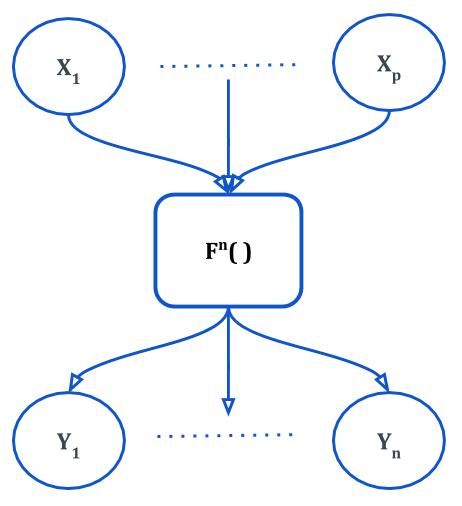
\includegraphics[width=0.5\textwidth]{method/data_preprocess/weather_data_preprocessing.jpg}
    \caption{Weather Data Preprocessing}
    \label{fig:weather_data_preprocessing}
\end{figure}
The WDIAS provides the support via in build simple generic mathematical function structure. Each extension is considering as a mathematical function which can take p 
number of input timeseries variables and output n number of timeseries variables. Other than that, at the time of processing the system can configure to provide
bind constant which can provide while configuring an extension. Which means, it is possible to change the behaviour of a existing function by providing different bind
constant at the time of creating new triggers for an extension.

\subsection{Interpolation}
The Interpolation module generates data at desired locations or at desired points in time by means of either a serial or spatial interpolation technique. It is applied for the filling in of data gaps in measured on-line data, as well as to derive spatially distributed data for meteorological time series, such as precipitation and temperature, based on information available at neighbouring locations.

\subsubsection{Serial Interpolation}
In serial interpolation mode, interpolation is done to fill any gaps in a time series. The interpolation module will only consider the time series itself in filling these gaps.
\begin{figure}[htp]
    \centering
    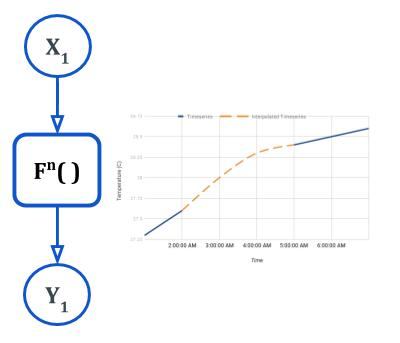
\includegraphics[width=0.6\textwidth]{method/data_preprocess/serial_interpolation.jpg}
    \caption{Serial Interpolation}
    \label{fig:serial_interpolation}
\end{figure}

\subsubsection{Spatial Interpolation}
In spatial interpolation mode, the interpolation can be either applied to fill gaps in time series, or to create a new time series for a location using data from other (spatially distributed) locations. Spatial interpolation can also be applied for sampling scalar time series from grid time series, for re-sampling grids, or for creating grids from time series data.
\begin{figure}[htp]
    \centering
    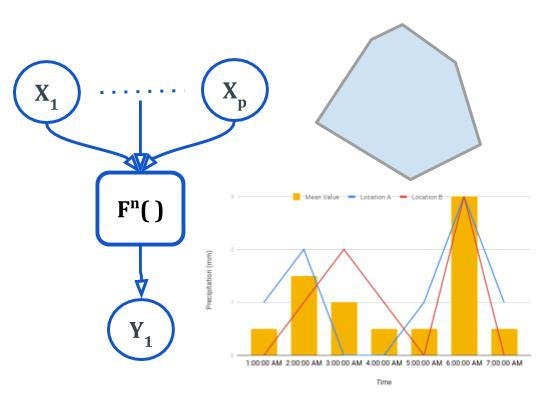
\includegraphics[width=0.6\textwidth]{method/data_preprocess/spatial_interpolation.jpg}
    \caption{Spatial Interpolation}
    \label{fig:spatial_interpolation}
\end{figure}

\subsection{Transformation}
Simple arithmetic manipulation, Time interval transformation and Shifting the series in time
Specific hydro-meteorological transformation such as stage discharge relationships
\begin{figure}[htp]
    \centering
    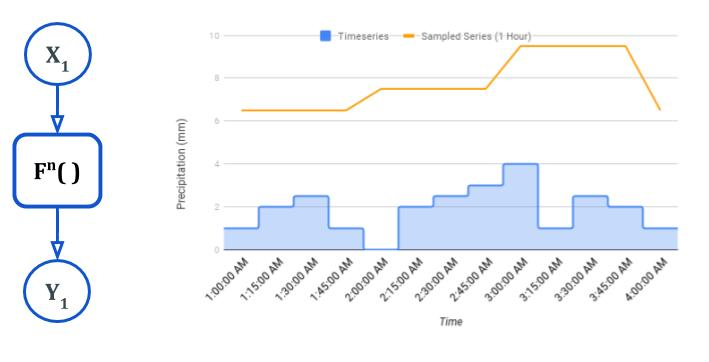
\includegraphics[width=0.6\textwidth]{method/data_preprocess/transformation.jpg}
    \caption{Transformation}
    \label{fig:transformation}
\end{figure}

\subsection{Validation}
Checks for counting reliable, doubtful, unreliable, and missing values
\begin{figure}[htp]
    \centering
    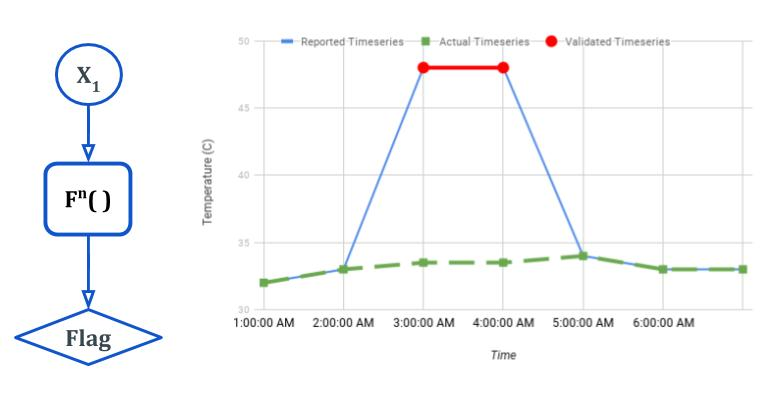
\includegraphics[width=0.6\textwidth]{method/data_preprocess/validation.jpg}
    \caption{Validation}
    \label{fig:validation}
\end{figure}

\subsection{Extension API}
In the WDIAS, it is possible to create new trigger for an extension via POST request to /extension endpoint.
\begin{lstlisting}[language=Python]
{
    "extensionId": "",
    "extension": "Interpolation/Transformation/Validation",
    "function": "",
    "variables": [
        {
            "variableId": "",
            "metadata/metadtaIds": {
            }
        }
    ],
    "inputVariables": [],
    "outputVariables": [],
    "trigger": [
        {
            "trigger_type": "OnChange/OnTime",
            "trigger_on": []
        }
    ],
    "options": {
    }
}
\end{lstlisting}
\begin{itemize}
    \item extensionId - An unique identifier for new extension trigger. Should be unique among all extensions.
    \item extension - The main extension category which is responsible for handling the extension with extracting data required and storing the output. Interpolation/Transformation/Validation support for the moment.
    \item function - Name of the microservice which is handling the input to output mapping. Fn() function in the \ref{fig:weather_data_preprocessing}.
    \item variables - Array timeseries mapping to variables. Multiple variables can be define with metadata or metadataIds of timeseries. Can be use same variable on inputVariables and outputVariables below.
    \item inputVariables - Timeseries that need to be provide into the function
    \item outputVariables - Timeseries that output from the function
    \item trigger - Type of trigger for the extension. Should be one of OnTime or OnChange.
    \begin{itemize}
        \item trigger - OnChange
        \item trigger\_on - List of timeseries to listen on change and trigger the extension
    \end{itemize}
    \begin{itemize}
        \item trigger - OnTime
        \item trigger\_on - List of schedules that need to be trigger the extension in cronjob string format
    \end{itemize}
    \item options - Bind Constant which is bind at the time of creating new extension trigger and pass on triggering the extension.
\end{itemize}

\subsubsection{Extension Handler}
Extension Handler is responsible for triggering the correct Extension with metadata when there is any change on subscribed extension trigger's OnChange timeseries.
\begin{figure}[htp]
    \centering
    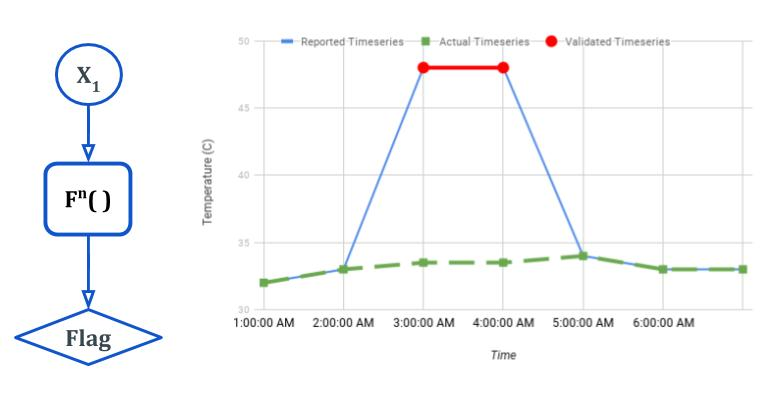
\includegraphics[width=0.6\textwidth]{method/data_preprocess/validation.jpg}
    \caption{Extension Handler}
    \label{fig:extension_handler}
\end{figure}

In further elaboration, when new data imported into one of adapter-scalar or adapter-vector, those notify the extension-handler. Then extension handler check whether there is any extension subscribed for particular timeseries, and trigger it via triggering an event on particular extensions.

In order to improve the performance of matching triggers against a timeseries, the WDIAS added two mechanisms. For the separation of service responsibilities, those functionalities reside in the adapter-extension and expose via an endpoint.
First, other than storing extension metadata in MySQL instance of adapter-extension, it also store the data in reverse lookup table called triggers. Using this reverse lookup table, for a given trigger\_type and timeseries, it can retrieve the extensions which are part of given timeseries. Thus the response which is received by the 
extension-handler only contains the extensions to be triggered. No additional filtering need to be done at the extension-handler service.
Second, cache the resulting trigger\_type and timeseries data in \acrshort{redis} database for fast access and avoid too much queries on \acrshort{mysql} database.

\subsubsection{Extension Scheduler}
Extension Handler is responsible for triggering the correct Extension with metadata at given time which is provided at the creation on extension trigger's with the value of OnTime cronjob string value.

In order to improve the performance of triggering cronjobs at given time schedules, the WDIAS added few optimization mechanisms.
Same as for extension-handler, the adapter-extension expose an endpoint to retrieve extension metadata grouped by cronjob time. Then use \acrshort{go} to implement the extension-handler to fast processing the extensions. After retrieve extension which are grouped by cronjob time; within the extension-handler, it schedules programatic cronjobs to trigger at given times. When each cronjob triggers at given time, it also contains the extensions to be triggered. Fetching extension data and creating cronjobs occur with long period of time in order to avoid heavy overhead.
When a new extension trigger created, those data push into a \acrshort{redis} List. Then pulling from the extension-handler in regular time intervals and create new cronjobs for mentioned cronjob time.
As mentioned above, in order to avoid the expansion of the programmatic cronjob list which are created for new extension triggers, all cronjobs fetch again in long period of time and flush the previously scheduled cronjobs.
The extension-handler should be run as a single entity for the atrocity, in order to avoid triggering same extension twice.